%!TEX root = main.tex

\documentclass[../main.tex]{subfiles}

\begin{document}

\chapter{Physical Measurements}
In this section, the physical measurements performed as part of the model development, will be described. These were done for two purposes. Some experiments are meant to recreate the results of the source papers which help confirm the theoretical aspects which inform the synthesis model (i.e. contact sound spectrum verification). Others were performed in an attempt to refine the model and make it more physically accurate as not all the synthesis parameters were physically informed in the source papers (i.e. $T_{60}$ values).

\section{Experimental Setup}
All tests were done on a Yahmaha-502 steel string acoustic guitar which was fitted with medium gauge D'Addario phosphor bronze strings. The strings were aged so their surface was rougher and less uniform as compared to a fresh set of strings. This was done because the sounds of aged strings are often considered more preferable on an acoustic guitar by many players. The slides used were Dunlop brass/chome/glass slides. Figure~\ref{fig:MySlides} contains a picture of the slides. The mass of the slides in descending order is: 125 grams (brass), 50.0 grams (chrome) and 17.5 grams (glass). 

\begin{figure}[h]
    \centering
    \includegraphics[scale=.15]{./images/pictures/MySlides.png}
    \caption{Slides used in the measurements}
    \label{fig:MySlides}
\end{figure}

The audio interface used was an RME Fireface UC. The microphones used were an AKG C480B and a DPA 4011-TL. The AKG was selected to be able to compare against the original measurements if need be as \citetwo{pakarinen_analysis_2007} and \citetwo{pakarinen_virtual_2008} list is as part of the experimental setup. The DPA 4011-TL was selected due to its flatter response which would allow more accurate measurements to be made. Contact microphones were considered as a potential option, however this was decided against as the extra mass they add to the guitar based on their placement could influence the measurements. The audio was captured at a sampling rate of 48,000 kHz using a MATLAB script to control the audio interface via ASIO.

For basic measurements (i.e. testing for the existence of of coupling), CIRMMT's \emph{A818 - Performance and Recording Lab} was used for measurements. When more precise measurements were required CIRMMT's \emph{A816 - Spatial Audio Lab} was used as it is a hemi-anechoic chamber.

\section{String Winding Density}
The first measurement made was to determine the linear string winding density for the different strings present on the guitar. This was done using a caliper set to a distance of 1 cm and taking a photo of it aligned with the beginning of a string winding through a magnifying glass. This allowed for the number of windings per centimeter to be counted which could then be multiplied by 100 to determine $n_w$, the density per meter, for each of the wound strings. Table~\ref{tab:WindingDensities} provides a summary of these measurements. Figure~\ref{fig:EWindings} illustrates the method for the E-string, while the Appendix contains the photos for all the strings measured.

\begin{table}[h]
\centering
    \begin{tabular}{||c|| c| c||} 
        \hline
        String & $\frac{\text{Windings}}{\text{cm}}$ & $\frac{\text{Windings}}{\text{m}}$ \\ [0.5ex] 
        \hline
        \hline
        \emph{E} & 20 & 2000 \\ 
        \hline
        \emph{A} & 26 & 2600 \\
        \hline
        \emph{D} & 38 & 3800 \\ 
        \hline
    \end{tabular}
\caption{Measured string winding densities}
\label{tab:WindingDensities}
\end{table}

\begin{figure}[h]
    \centering
    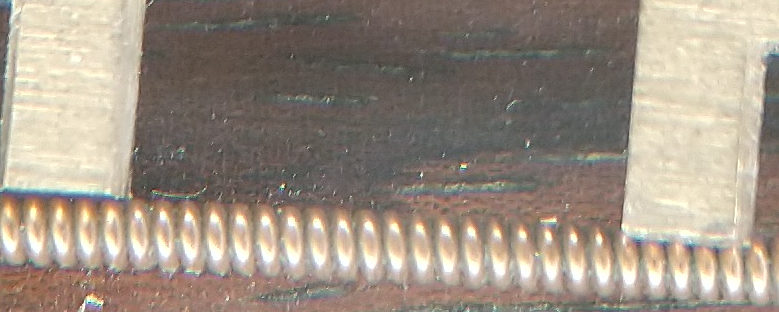
\includegraphics[scale=.75]{./images/pictures/WindingsEZoom.png}
    \caption{E-string winding density measurement. The distance between the inner edges of the caliper is 1 cm.}
    \label{fig:EWindings}
\end{figure}

\section{Transverse to Longitudinal Coupling}
The original model assumes coupling between the longitudinal motion of the slide and transverse vibrations of the strings. This is indicated by the injection of the CSG out into the string DWG structure as shown in Fig.~\ref{fig:original_DWG}. Two potential sources for this coupling are due to reflections from an imperfect bridge impedance as well as imperfections in the slide/winding collisions, or friction between the string/slide surface (especially in the case of the unwound strings). The goal of these measurements is to confirm that the coupling exists and qualitatively determine the strength to facilitate rough comparisons across different string and slide combinations. These measurements were performed in \emph{A818} as the the precision required for a successful experiment did not require the less reflective attributes of \emph{A816}.

\subsection{Setup and Method}
The general method for testing the coupling on a string is described as follows. First, the other strings were muted with ear plugs to prevent any sort of sympathetic vibrations or other unwanted coupling. The slide was held in the left hand and the right hand was used to dampen the string while the slide was placed on it. This was done as the initial contact between the slide and string often creates a click/impulse, which is unwanted in this case. The muting helps ensure that there are no vibrations in the string before the slide moves. After ensuring the system would be starting from rest, the slide was moved along the string from the 7th fret up to the 12th and back. This motion was repeated twice in a recording. The mic was placed over the 12th fret as this produced the best results. Figure~\ref{fig:CouplingSetup} shows a photograph of the setup.

\begin{figure}[h]
    \centering
    \includegraphics[scale=.20]{./images/pictures/CouplingSetup.png}
    \caption{Setup used to confirm longitudinal-to-transverse coupling. Ear plugs are used to mute strings not being measured.}
    \label{fig:CouplingSetup}
\end{figure}

\subsection{Results}
For all the strings it was confirmed that coupling between the longitudinal slide motion and transverse vibrations of the strings exists. Figure~\ref{fig:L2CSpectrum} illustrates this for the brass slide being moved along the low E-string. The recording used to generate this plot can be heard in \emph{CouplingMeasurement-E-string-Brass.wav}. As can clearly be observed in the plot and heard on the recording, the appropriate harmonics of the transverse vibrations corresponding to the slide's placement along the string are being stimulated by the slide's longitudinal motion.

\begin{figure}[h]
    \centering
    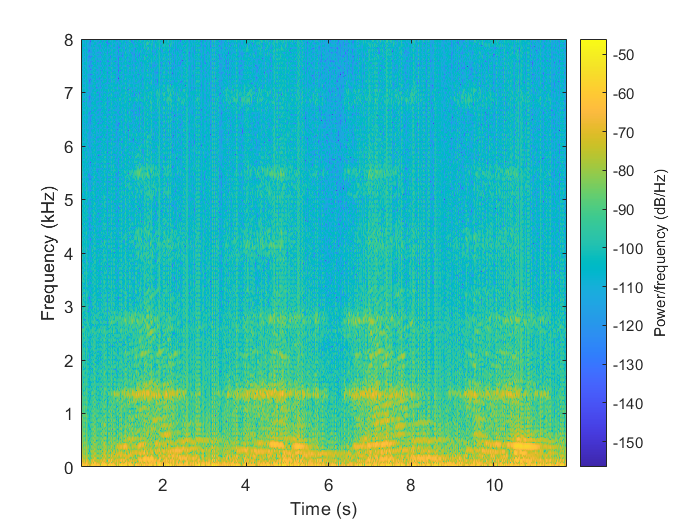
\includegraphics[scale=.75]{./images/plots/EBrassCoupling.png}
    \caption{Spectrogram of coupling measurements for the brass slide moved along the E-string}
    \label{fig:L2CSpectrum}
\end{figure}

Two patterns were observed relating the strength of the coupling to the slide used as well as the string. For a specific string, the slides produced coupling from greatest to least in the following order: brass, chrome and glass. This order corresponds to listing the slides in order from heaviest to lightest as well as roughest to smoothest. Intuitively this makes sense as the heavier slides have more mass and would proportionally transfer more energy to the string on each slid/winding collision as compared to the lighter slides. The same would apply from a friction standpoint, where the rougher surfaces would provide more opportunities to create kinetic friction and transfer energy into the string.

When comparing the coupling across different strings for the same slide type, the pattern observed was that the strings produced coupling from greatest to least in the following order: E, A, D, G, B and e. The first four are wound strings, and in order of decreasing winding size. The pattern could be explained by the fact that the larger windings provide more surface area to collide with allowing more coupling to be generated. In terms of the unwound strings, a similar argument could be made regarding the thickness of the string providing more surface area for the slide to interact with. However, given the strings are rather old and exhibit corrosion, it is hard to definitively conclude the coupling source regarding the unwound strings.

\section{Contact Noise Spectrum}
\subsection{Method}
The contact noise spectrum measurements were done in the \emph{Spatial Audio Lab}. Ear plugs and window sealing foam were used to mute the transverse vibrations of the string being measured. As one side of the foam was adhesive, a strip of tape was applied to ensure the fretboard wouldn't be damaged be the adhesive. The other strings were muted with the right hand near the sound hole while the measurement was being performed. Figure~\ref{fig:FoamStrip} illustrates foam muting technique.

\begin{figure}[h]
    \centering
    \includegraphics[scale=.15]{./images/pictures/FoamDamping.png}
    \caption{A foam strip placed underneath the E string to dampen its transverse vibrations. Note how the string protrudes nicely without sinking too far into the foam.}
    \label{fig:FoamStrip}
\end{figure}

In order to mitigate the non-deterministic aspect of a human controlled slide, the following approach was used. A metronome was set to 100 bpm to provide a consistent pulse. The slide was then moved up one length on a beat and then down the same length the following beat, with the up-down pattern performed twice in a row for each set of frets. The first distance was defined by frets 5 \& 7, the second by frets 5 \& 9 and the third by frets 5 \& 12. These different distances were selected to have the top speed reached by the slide increase on each measure.

\subsection{Results}
Figure~\ref{fig:ContactNoiseEBrass} illustrates a spectrogram of  measurements from the DPA microphone for the experiment being performed on the low E string with the brass slide. This can be heard in the file \emph{NoiseCharacterization-E-brass.wav}. The results are extremely similar to the analysis performed in \citetwo{pakarinen_virtual_2008} for the slide guitar and \citetwo{pakarinen_analysis_2007} for finger noises. There are clearly both the time-varying harmonic as well as static modal components to the sound. It is also quite clear that the fundamental frequency of the harmonic varies with the slide velocity. What wasn't made clear in the previous work though, is that it appears as if there are higher longitudinal harmonics whose strength is correlated with the magnitude of the slide velocity. They appear all throughout the spectrum but are most strongly stimulated around ~9 and 8.5 kHz and reach all the way to the upper end of the spectrum near ~23.4 kHz and ~23.8 kHz when the slide is moving fastest. The previous work did not attempt to control for the slide speed as much, which is a possible explanation as to why this wasn't mentioned.

\begin{figure}[h]
    \centering
    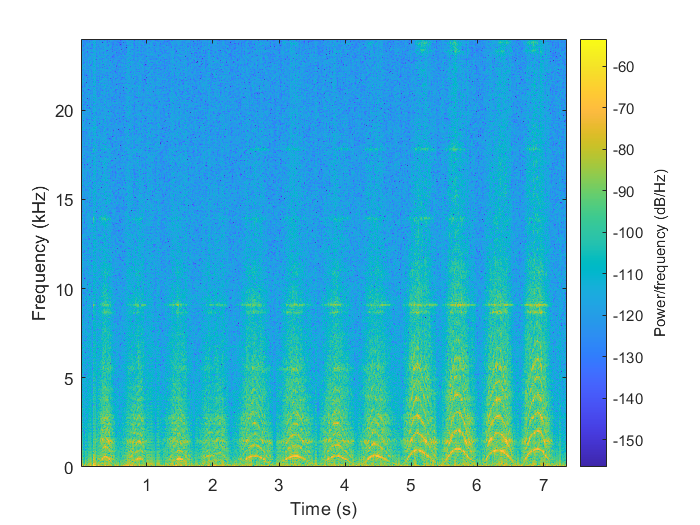
\includegraphics[scale=.65]{./images/plots/ContactNoiseEBrass.png}
    \caption{Measured spectrum for brass slide on E string. A 12 ms rectangular window with 75\% overlap was used.}
    \label{fig:ContactNoiseEBrass}
\end{figure}

It was difficult to perform this measurement on the unwound strings as they had a tendency to sink into the foam more so than the wound strings. As a result the slide would make contact with the protruding foam. This simultaneously made it difficult to move the slide in a consistent and repeatable manner as well as introduced its contact sound due to the noise between the foam and the slide. An attempt was made to cut the foam into a thinner strip to reduce the protrusions, but this was difficult to do uniformly and the same problem was exhibited. Figure~\ref{fig:CutFoam} shows the results of this attempt. Accordingly, the parameters of the synthesis model for unwound strings could not be as precisely confirmed.

\begin{figure}[h]
    \centering
    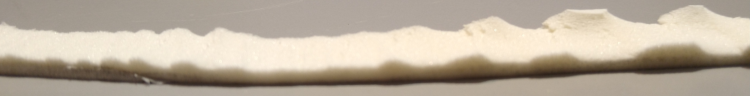
\includegraphics[scale=.15]{./images/pictures/CutFoam.png}
    \caption{A failed attempt to reduce the thickness of the foam.}
    \label{fig:CutFoam}
\end{figure}

\section{Decay Rate of Single Winding Impact}
\label{sec:DecayRateMeasurement}
Based on the material in \citetwo{pakarinen_virtual_2008} and \citetwo{puputti_real-time_2010}, it is unclear as to how the values for the decay rate associated with the noise pulses were obtained. Two methods were investigated in an attempt to derive a more physically informed value for these parameters. In either case it is not necessary to know the input force precisely, as the relative changes in signal strength over time are what is of interest. This drastically reduces the complexity of the tools required in the physical setup. The foam used for muting would likely impede the longitudinal motion of the string slightly and as it is also used in the noise characterization setup then the same effect would be seen in both experiments. Given this experiment will ultimately be used to inform the tuning process by ear, it isn't necessary to have the most precise method. The small amount of error the foam introduces is acceptable as it narrows down the search range of tuning parameters later on and provides a solid starting point.

\subsection{Methods}
Both methods here rely on an assumption of linearity. In both setups, the string being measured was muting using the foam strips as in the contact sound experiments. The object used to stimulate the strings was an utility knife blade removed from its casing. Attempts were made to use it inside the casing, however this setup didn't provide the same rigidity as when removed from the case. The interaction between the knife edge and the string windings is different than the slide and string, however the assumption of linearity  allows the results to be generalized. Additionally the goal here isn't to develop a precise characterization, but have a stronger physical basis for the $T_{60}$ parameter used to control the synthesizer. 

\subsubsection{Hold and Release}
Figure~\ref{fig:KnifeEdgeWedge} shows a photograph of a preliminary experimental setup before the knife was removed from the casing and the muting foam was added. In this setup the knife's edge was wedged between two string windings. From there, force was applied in the longitudinal direction until slippage occurred and the knife edge dislodged from the string winding. At this point all the potential energy stored in the string longitudinally would start to release and be exchanged into kinetic energy, starting the oscillation process. Capturing this process would ideally allow the system's overall decay rate to be measured and used to tune the model.

\begin{figure}[h]
    \centering
    \includegraphics[scale=.2]{./images/pictures/KnifeEdgeWedge.png}
    \caption{Knife edge wedged in between two string windings. This method was revised to be done with the blade out of the casing and on a string muted with foam.}
    \label{fig:KnifeEdgeWedge}
\end{figure}

\subsubsection{Strike Multiple Windings}
Figure~\ref{fig:KnifeStrikingSetup} illustrates the experimental setup for this case. The setup is extremely similar to the previous one, except for in this case the knife edge was held at an angle. Changing the position in this manner would allow it to more easily slide across the winding surface. This is desirable in this case as the goal is to strike a small number of windings sequentially and extract the $T_{60}$ parameter from the resulting signal which either contains overlapped impulse responses or several individual ones depending on the relationship between the knife-edge velocity and duration of the impulse responses. The approach was developed based on difficulties in controlling the physical setup in the previously designed experiments.

\begin{figure}[h]
    \centering
    \includegraphics[scale=.18]{./images/pictures/KnifeStrikingSetup.png}
    \caption{Knife striking setup. Alternating strings have muting foam as it was easier to prepare the setup for the next string measurements.}
    \label{fig:KnifeStrikingSetup}
\end{figure}

\subsection{Results}
\label{sec:T60Measurement}
Unfortunately neither of the two methods did not work as exactly as hoped due to the noise floor of the measurement system. However, the results can be used to help determine a starting point from which to begin tuning the $T_{60}$ parameter for each string as well as providing values to compare against the ones listed in Fig. B.6 of \cite{puputti_real-time_2010} where the implementation is described.

Figure~\ref{fig:T60Measurement} illustrates the strongest peak for the low E string which was obtained from the single winding measurements. The data has been normalized to make it easier to find the point at which it decays to .001. Unfortunately, due to the noise in the system this exact value was not able to be found easily. However, an extremely rough measurement of $T_{60}$ can be obtained by estimating the point at which the noise becomes strongest after the peak. Based on the values shown in the graph, this results in a measured $T_{60}$ value of approximately 20.4 ms. Clearly this measurement is extremely rough and not the most precise or accurate, however for the same string \citetwo{puputti_real-time_2010} lists a value of 200 ms. The measured value is roughly an order of magnitude smaller and as the method by which the parameter values were obtained is not elaborated upon in the source material, it provides a stronger physical basis from which to begin tuning the parameter.

\begin{figure}[h!]
    \centering
    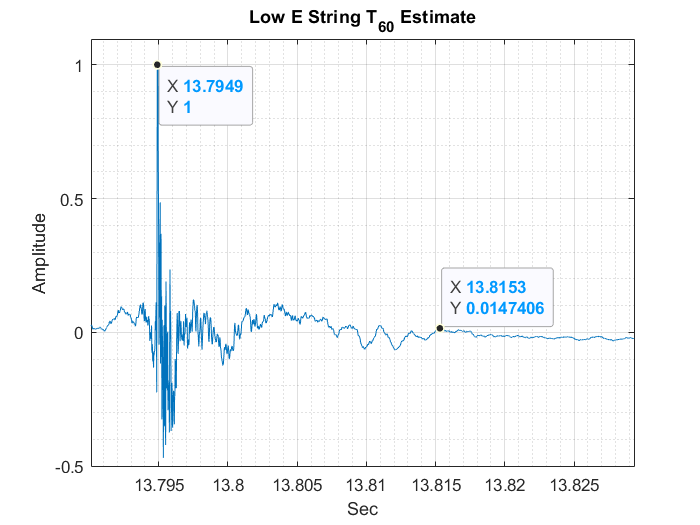
\includegraphics[scale=.60]{./images/plots/T60Attempt.png}
    \caption{Plot of the strongest peak for the single winding experiment on the low E string which is used to roughly estimate $T_{60}$. The estimate here puts $T_{60}$ at approximately .0204 seconds.}
    \label{fig:T60Measurement}
\end{figure}

\clearpage

\section{Playing Examples}
 The last measurements made were recordings of a particular slide example. This was done to be able to capture real-world examples for comparison to the synthesized examples. The spectral aspects of the sound are useful from the standpoint of determining the parameters of the synthesis model (i.e. balance between the longitudinal modes and harmonic component of wound string contact sounds). The fundamental frequency as a function of time is also of interest as this can be used to inform the $L[m]$ control signal to make the articulations more realistic. This will be discussed more in the subsequent chapter on sound design.
\end{document}